%%%%%%%%%%%%%%%%%%%%%%%%%%%%%%%%%%%%%%%%%
% Beamer Presentation
% LaTeX Template
% Version 1.0 (10/11/12)
%
% This template has been downloaded from:
% http://www.LaTeXTemplates.com
%
% License:
% CC BY-NC-SA 3.0 (http://creativecommons.org/licenses/by-nc-sa/3.0/)
%
%%%%%%%%%%%%%%%%%%%%%%%%%%%%%%%%%%%%%%%%%

%----------------------------------------------------------------------------------------
%	PACKAGES AND THEMES
%----------------------------------------------------------------------------------------

\documentclass{beamer}

\mode<presentation> {

% The Beamer class comes with a number of default slide themes
% which change the colors and layouts of slides. Below this is a list
% of all the themes, uncomment each in turn to see what they look like.

%\usetheme{default}
%\usetheme{AnnArbor}
%\usetheme{Antibes}
%\usetheme{Bergen}
%\usetheme{Berkeley}
%\usetheme{Berlin}
%\usetheme{Boadilla}
%\usetheme{CambridgeUS}
%\usetheme{Copenhagen}
%\usetheme{Darmstadt}
%\usetheme{Dresden}
%\usetheme{Frankfurt}
%\usetheme{Goettingen}
%\usetheme{Hannover}
%\usetheme{Ilmenau}
%\usetheme{JuanLesPins}
%\usetheme{Luebeck}
\usetheme{Madrid}
%\usetheme{Malmoe}
%\usetheme{Marburg}
%\usetheme{Montpellier}
%\usetheme{PaloAlto}
%\usetheme{Pittsburgh}
%\usetheme{Rochester}
%\usetheme{Singapore}
%\usetheme{Szeged}
%\usetheme{Warsaw}

% As well as themes, the Beamer class has a number of color themes
% for any slide theme. Uncomment each of these in turn to see how it
% changes the colors of your current slide theme.

%\usecolortheme{albatross}
%\usecolortheme{beaver}
%\usecolortheme{beetle}
%\usecolortheme{crane}
%\usecolortheme{dolphin}
%\usecolortheme{dove}
%\usecolortheme{fly}
%\usecolortheme{lily}
%\usecolortheme{orchid}
%\usecolortheme{rose}
%\usecolortheme{seagull}
%\usecolortheme{seahorse}
%\usecolortheme{whale}
%\usecolortheme{wolverine}

%\setbeamertemplate{footline} % To remove the footer line in all slides uncomment this line
%\setbeamertemplate{footline}[page number] % To replace the footer line in all slides with a simple slide count uncomment this line

%\setbeamertemplate{navigation symbols}{} % To remove the navigation symbols from the bottom of all slides uncomment this line
}
\usepackage{graphicx} 
\usepackage{animate}% Allows including images
\usepackage{booktabs} % Allows the use of \toprule, \midrule and \bottomrule in tables
\usepackage{float} 
\usepackage{color}
\definecolor{light}{rgb}{0.5, 0.5, 0.5}
\def\light#1{{\color{light}#1}}

%----------------------------------------------------------------------------------------
%	TITLE PAGE
%----------------------------------------------------------------------------------------

\title{Machine Learning Project Life Cycle} % The short title appears at the bottom of every slide, the full title is only on the title page

\author{Yapi Donatien Achou} % Your name
\institute[Semcon] % Your institution as it will appear on the bottom of every slide, may be shorthand to save space
{
Semcon \\ % Your institution for the title page
\medskip
\textit{yapi-donatien.achou@semcon.com} % Your email address
}
\date{\today} % Date, can be changed to a custom date

\begin{document}

\begin{frame}
\titlepage % Print the title page as the first slide
\end{frame}

\begin{frame}
\frametitle{Overview} % Table of contents slide, comment this block out to remove it
\tableofcontents % Throughout your presentation, if you choose to use \section{} and \subsection{} commands, these will automatically be printed on this slide as an overview of your presentation
\end{frame}

%----------------------------------------------------------------------------------------
%	PRESENTATION SLIDES
%----------------------------------------------------------------------------------------

%------------------------------------------------

\section{Machine learning/data science project life cyle}
\begin{frame}
\frametitle{Machine learning/data science project life cyle}
\begin{figure}[H] %  figure placement: here, top, bottom, or page
   \centering
   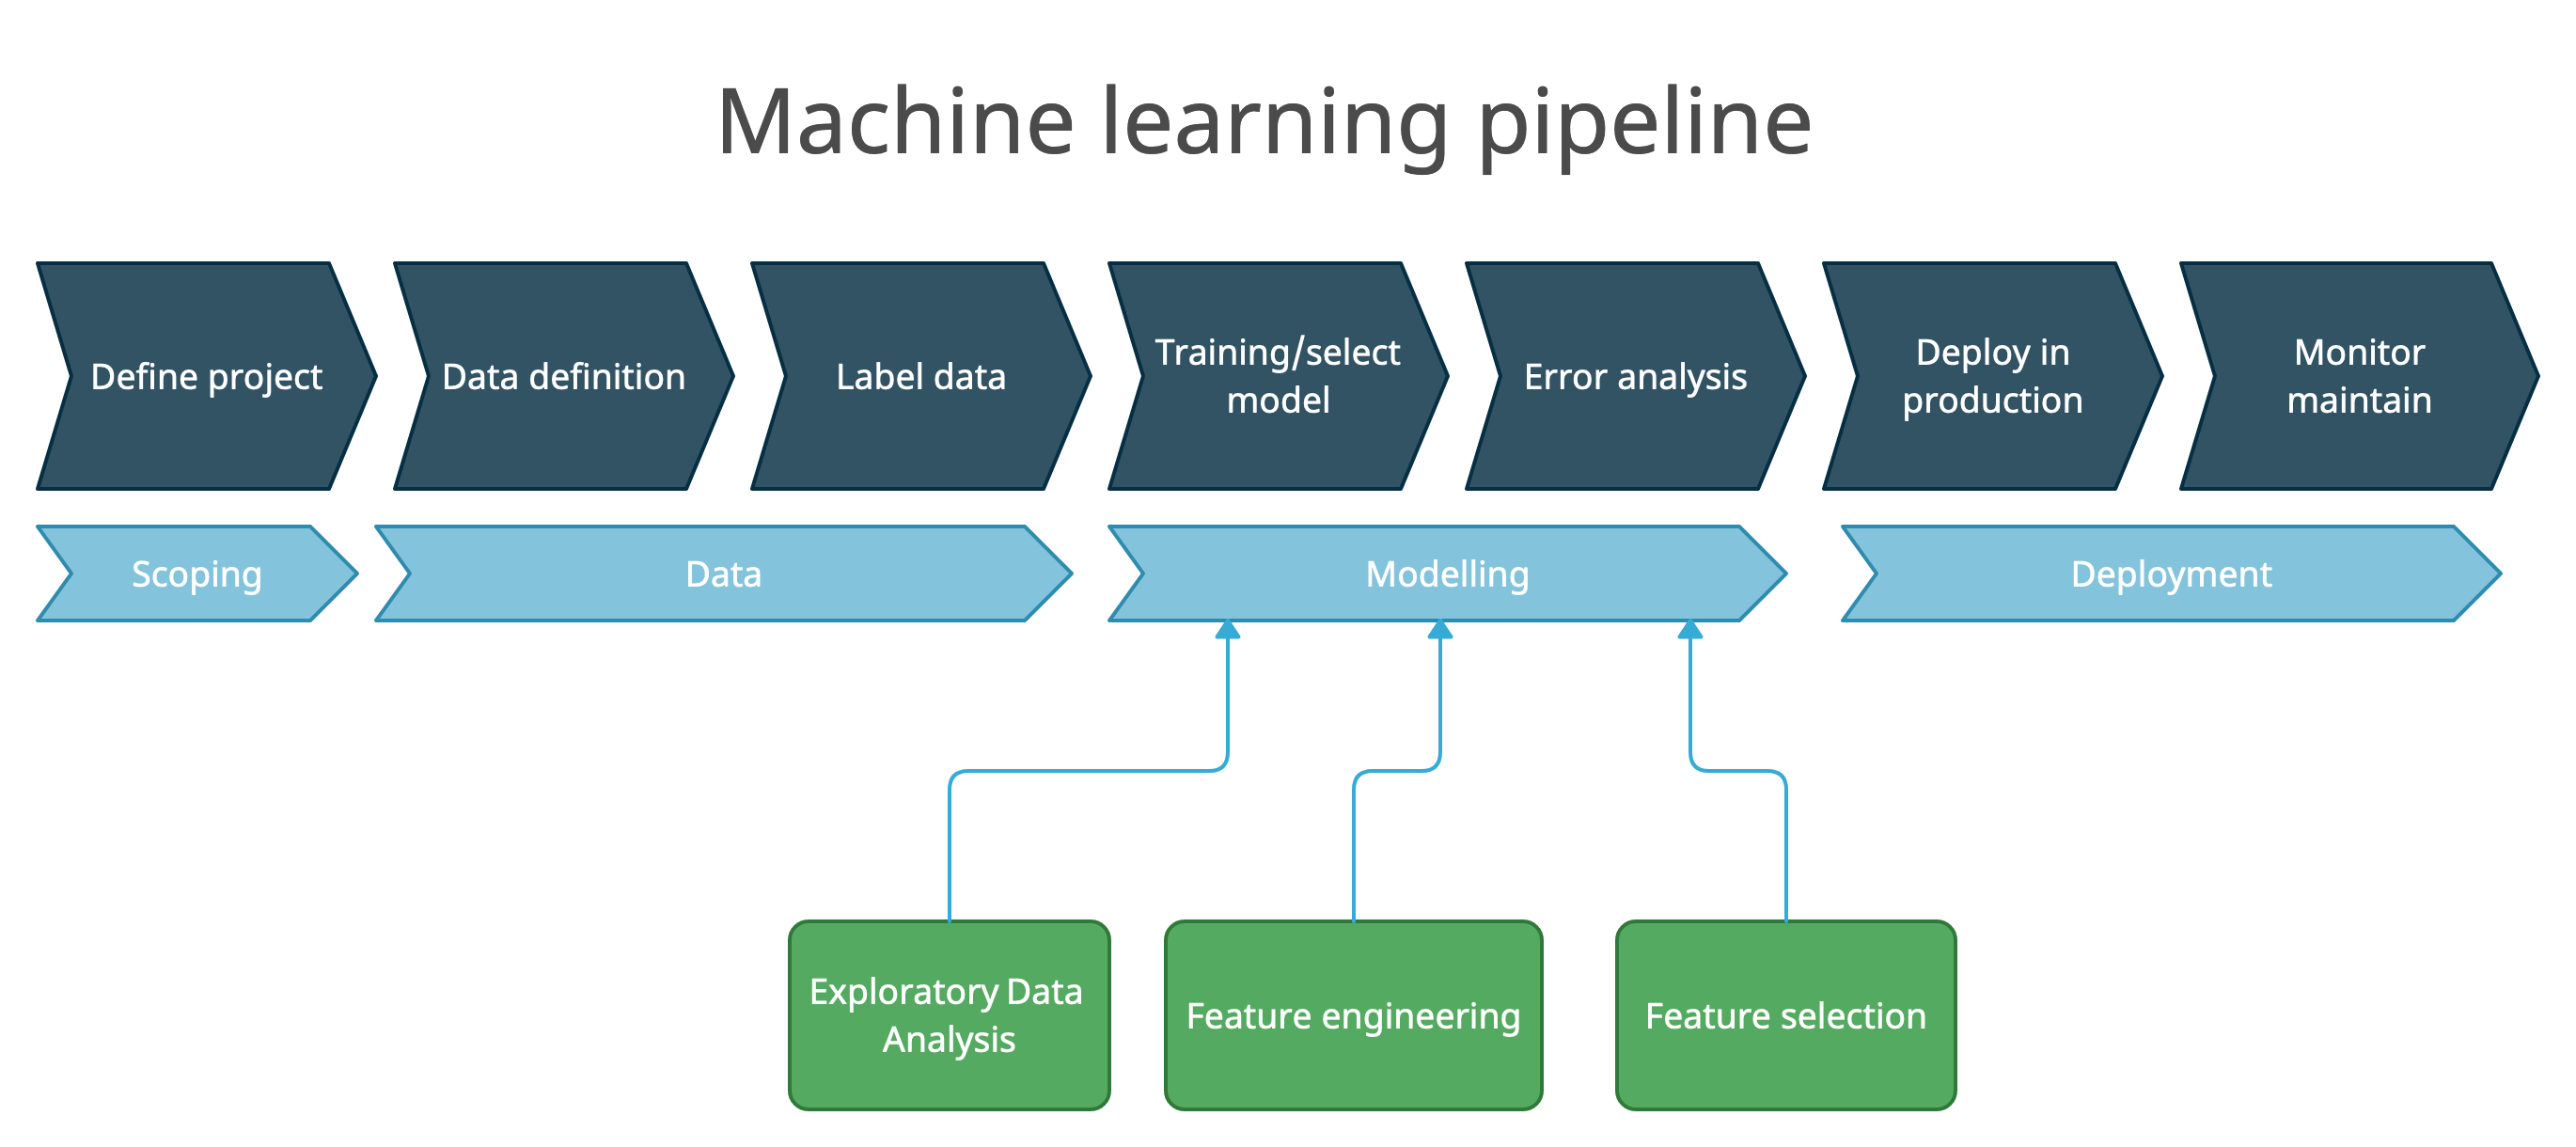
\includegraphics[width=5in]{figures/ml-pipeline.png} 
\end{figure}
\end{frame}


%------------------------------------------------
%------------------------------------------------


\section{Machine learning paradigm}
\begin{frame}
\frametitle{Machine learning paradigms}
\begin{block}{Supervised learning}
\begin{figure}[H] %  figure placement: here, top, bottom, or page
   \centering
   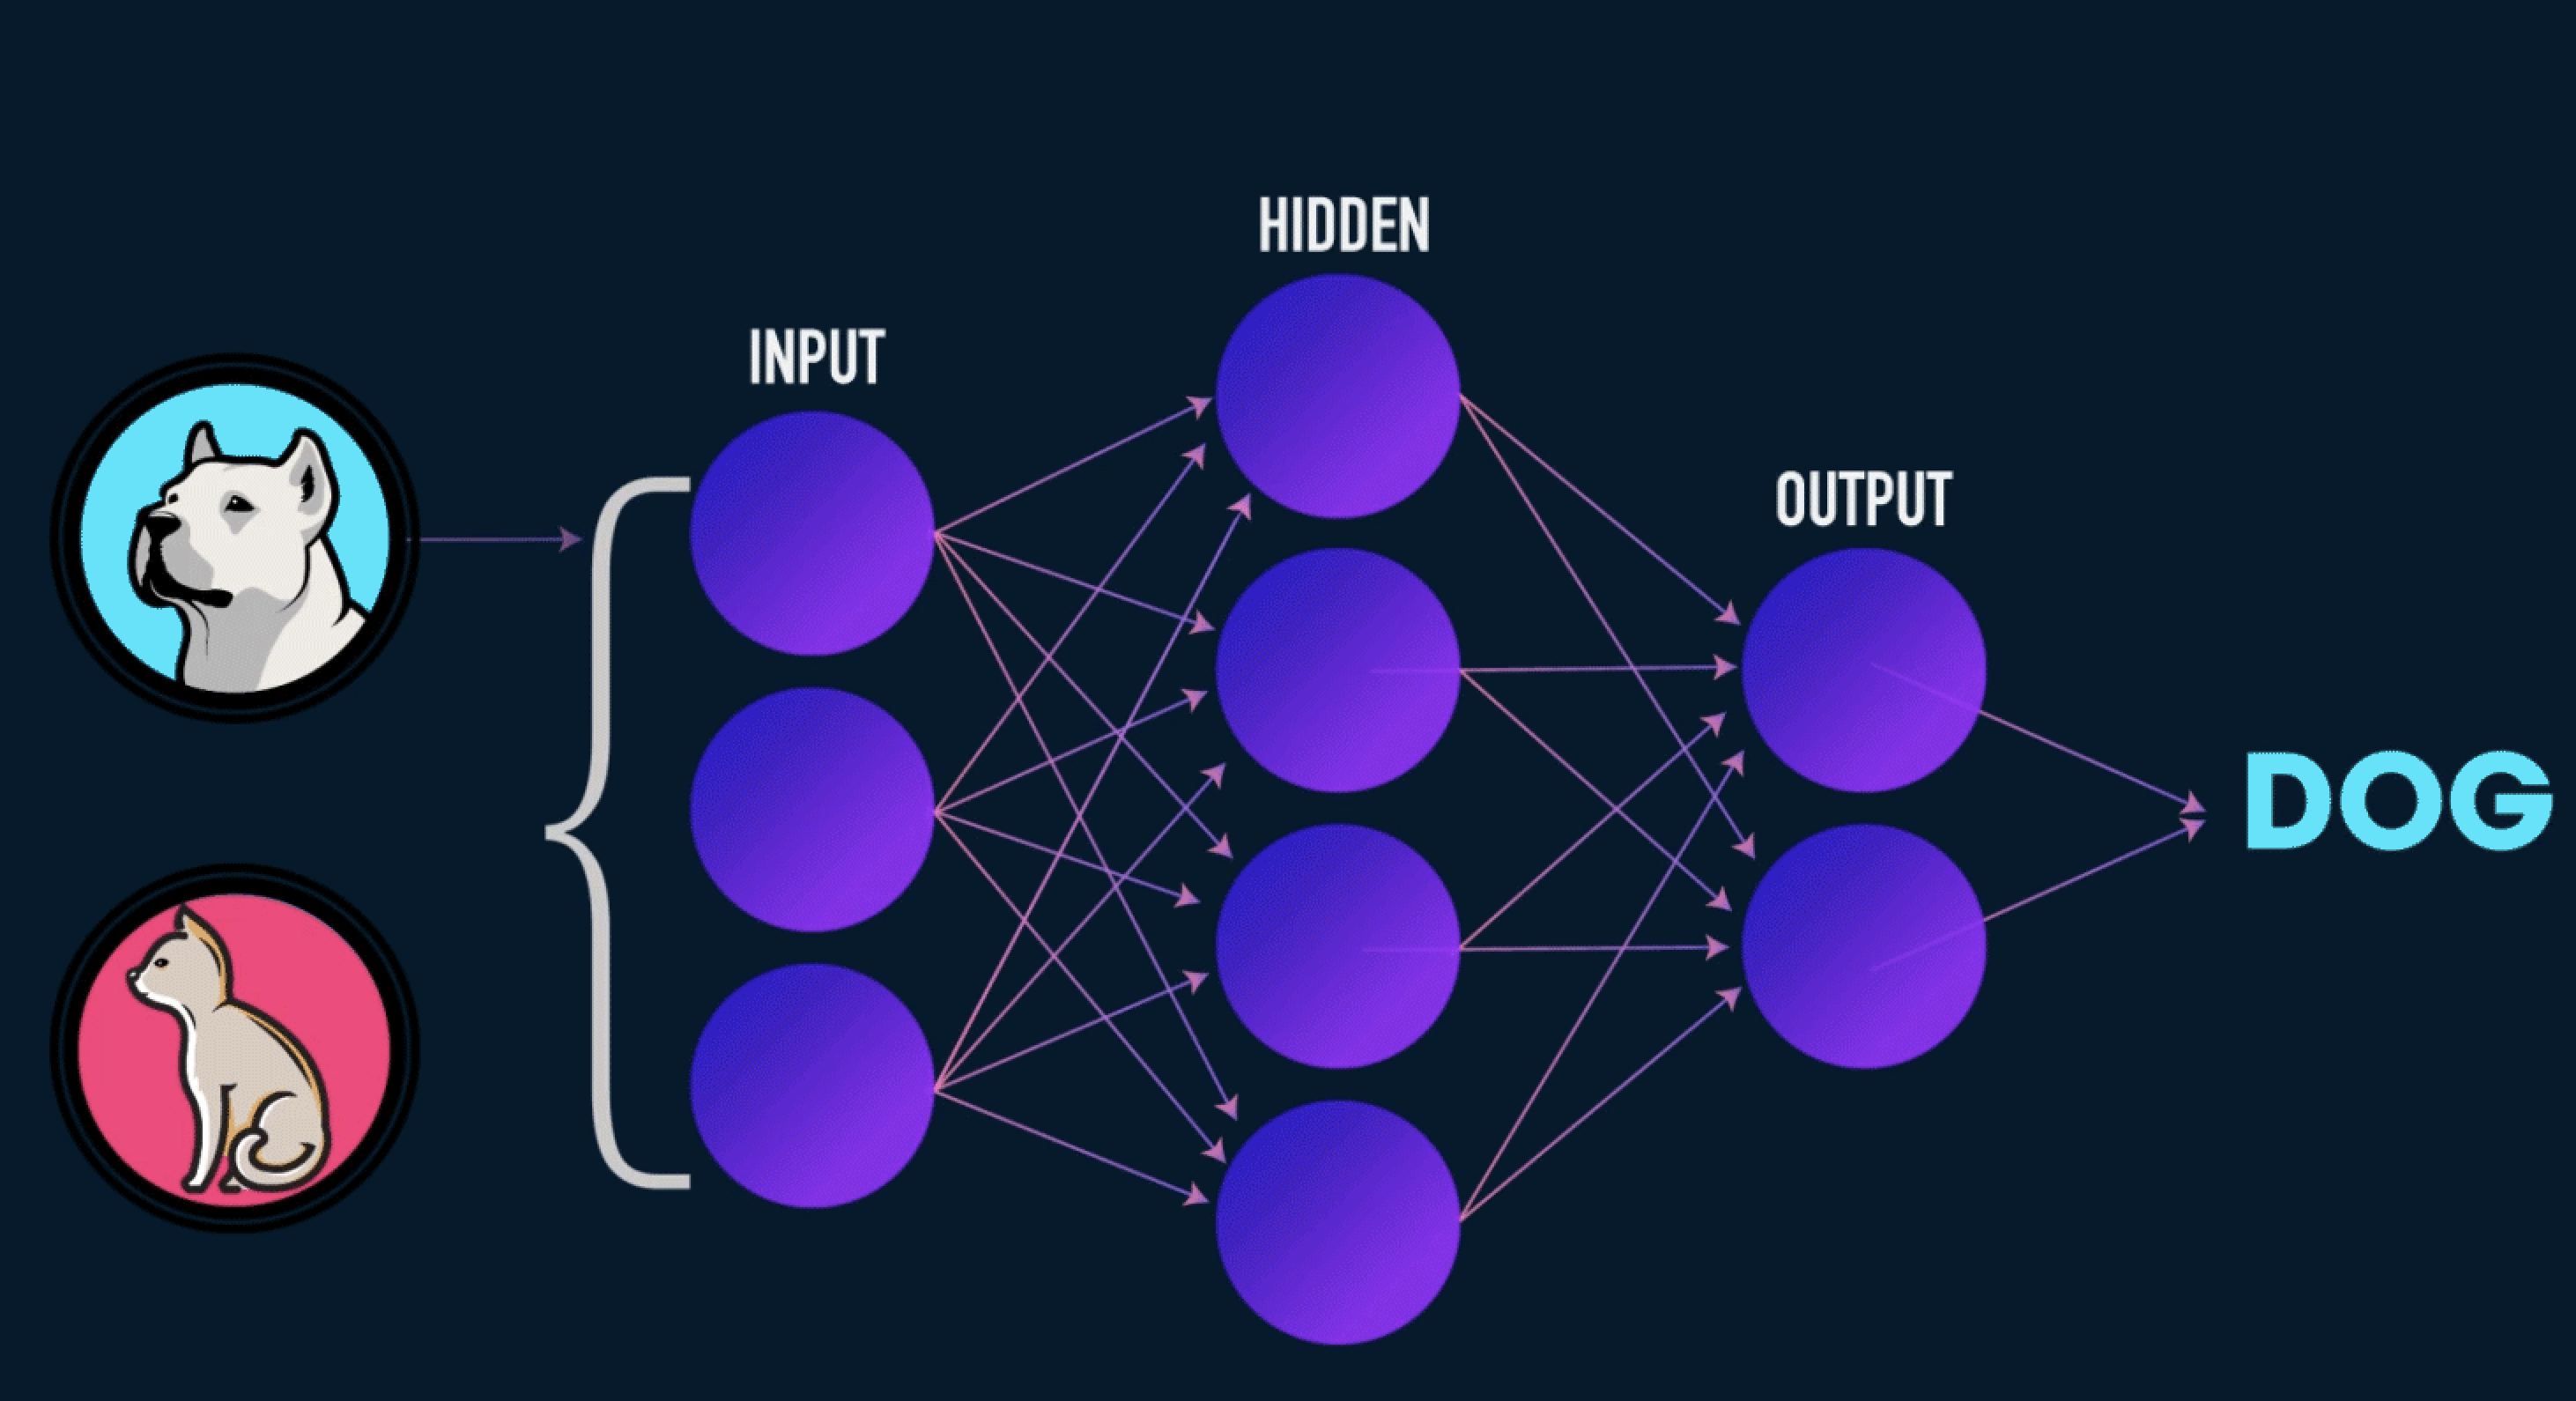
\includegraphics[width=4in]{figures/supervise-learning.png} 
\end{figure}
\end{block}
\end{frame}
%--------------------------------------------------
\begin{frame}
\frametitle{Machine learning paradigms}
\begin{block}{Unsupervised learning}
\begin{figure}[H] %  figure placement: here, top, bottom, or page
   \centering
   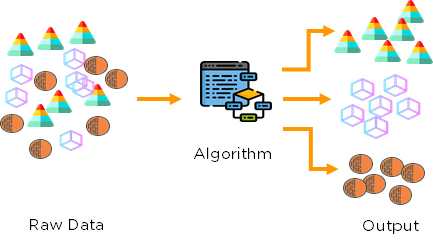
\includegraphics[width=4in]{figures/unsupervise-learning.png} 
\end{figure}
\end{block}
\end{frame}

%------------------------------------------------
%------------------------------------------------
\section{Introduction to neural networks with Tensorflow/keras} 
\begin{frame}
\frametitle{Introduction to Multi Layer Perceptron (MLP) with Tensorflow/Keras}
\begin{figure}[H] %  figure placement: here, top, bottom, or page
   \centering
   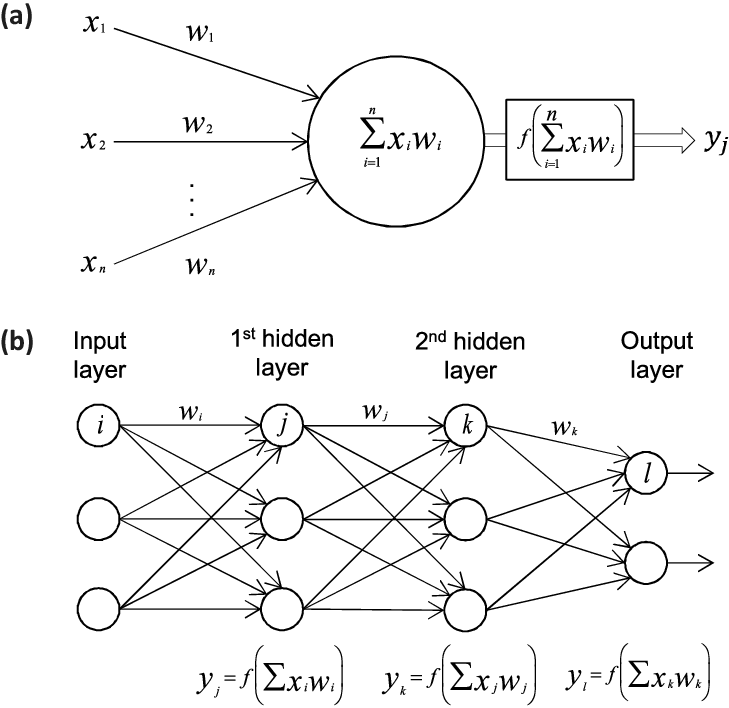
\includegraphics[width=2.8in]{figures/mlp.png} 
\end{figure}
\end{frame}

\begin{frame}
\frametitle{Introduction to Convolutional Neural Network (CNN) with Tensorflow/Keras}
\begin{figure}[H] %  figure placement: here, top, bottom, or page
   \centering
   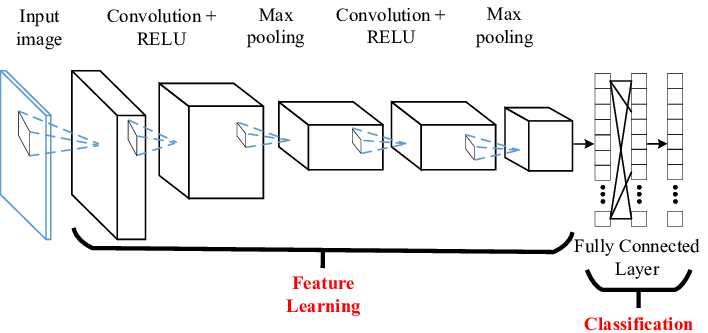
\includegraphics[width=4.5in]{figures/cnn.png} 
   \end{figure}
\end{frame}

%------------------------------------------------
%------------------------------------------------
%------------------------------------------------
\section{Example projects with Tensorflow/Keras}
\begin{frame}
\frametitle{Project 1: Classification}
\begin{example}
\begin{enumerate}
\item Build the model architecture 
\item Select the loss function
\item Select your learning algorithm
\item Iteratively train the model
\item \light{Deploy model to production}
\item \light{Use model in production}
\end{enumerate}
\end{example}
\end{frame}

\begin{frame}
\frametitle{Project 2: Classification and regression}
\begin{example}
\begin{enumerate}
\item Build the model architecture 
\item Select the loss function
\item Select your learning algorithm
\item Iteratively train the model
\item \light{Deploy model to production}
\item \light{Use model in production}
\end{enumerate}
\end{example}
\end{frame}


\begin{frame}
\frametitle{Project 3: Image segmentation}
\begin{example}
\begin{enumerate}
\item Build the model architecture 
\item Select the loss function
\item Select your learning algorithm
\item Iteratively train the model
\item \light{Deploy model to production}
\item \light{Use model in production}
\end{enumerate}
\end{example}
\end{frame}


\end{document} 